%\documentstyle[graphicx,natbib]{article}
\documentclass[11pt]{article}
\usepackage{aas_macros}
\usepackage{graphicx}
\usepackage[numbers]{natbib}
\usepackage{hyperref}


\setlength{\parskip}{2ex}
\setlength{\parindent}{2em}
\setlength{\textwidth}{16cm}
\setlength{\textheight}{23cm}
\setlength{\oddsidemargin}{0.25cm}
\setlength{\evensidemargin}{0.25cm}
%\setlength{\topmargin}{-2.0cm}         % Zurich
\setlength{\topmargin}{-1.5cm}         % Bern
\def\thefootnote{\fnsymbol{footnote}}

\setlength{\parindent}{0pt} % No indent

\renewcommand{\thesection}{\Alph{section}}
\renewcommand{\thesubsection}{\arabic{subsection}}


%\def\mnras{\ref@jnl{MNRAS}}


%-----------------------------------------------------------------------

\begin{document}

\newpage

\section*{Research Plan}

\begin{abstract}
Blabla
\end{abstract}


\subsection{Introduction and Status of Research}

\subsubsection{General relativity and gravitational lenses}

In the year 1915, Albert Einstein published the theory of General Relativity (GR).
This theory describes the interplay of matter (energy and impulse) and space-time and the perturbations on the latter caused by the former.
GR allowed the first time to correctly describe the anomalous precession of Mercury.
The next experimental proof of GR was the deflection of the light of a star by the sun (by Eddington in the year 1919).
Einstein already predicted this phenomena in 1911 up to a factor of two.
This was the starting shoot for Einstein’s second great theory and first observation and evidence of \emph{(micro) gravitational lensing}\footnote{Even thou the accuracy of this measurement was questioned, see\cite{kennefick2009testing}}.

Gravitational Lensing (GL) describes the phenomena of deflection of light around a massive object, due to the deflections in space-time caused by the mass.
Quite similar to the deflection of the path of a marble rolling on a rubber sheet, stretched by a mass in it's centre.
If the source of the light (``source''), the massive object (``lens'') and the observer align approximately in a line, these distortions act similar to a regular lens.
Depending on the configuration, a background light source is distorted, magnified or even multiplied, as shown in Fig.~\ref{fig:grav_lens}.

\begin{figure}[h]
	\centering
		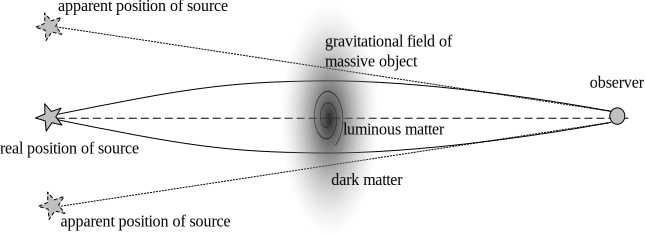
\includegraphics[width=0.75\textwidth]{img/grav_lens}
	\caption{Schematics of gravitational lensing}
	\label{fig:grav_lens}
\end{figure}

This phenomena is divided into three sub phenomena:
\begin{itemize}
	\item \emph{Strong lensing} occurs if the lens is extremely massive. Consider a single galaxy, galaxy clusters or black holes.
Strong lensing allows not only for displacements of sources, but for magnification and creation of multiple images.
The first observed strong lensing was the twin quasar Q0957+561 discovered 1979 (\cite{walsh19790957}).
  \item In contrast, \emph{Weak lensing} phenomena are not directly observable.
The GL caused by a weak or far away gravitational field causes only a distortion of the shape of sources (shear), that can be statistically analysed.
  \item \emph{Micro lensing} deals with tiny perturbations of the perceived light magnitude from a source, caused by gravitational field in the order of single lensing stars.
Micro lensing is used to detect MACHOs\footnote{Massive Astrophysical Compact Halo Object} and extra solar planets.
\end{itemize}

In my work, I'm focussing on strong lensing, since it's directly detectable in astronomical pictures taken by telescopes.


\subsubsection{Gravitational lens modelling}

Since the effect of gravitational lensing depends on a variety of parameters, the study of gravitational lenses allow an alternative approach of estimating many of those parameters.
The study of a discovered gravitational lens usually involves in a first step to create an accurate model for the source light profile / distribution, the lensing mass distribution and the distances between source, lens and observer.
This process is commonly referred to as ``modelling'' a gravitational lens.
These models allow to tackle down a lot of open questions in current astrophysics and even some general physical questions.

The model of the lensing allows in a first step to estimate total masses of distant (lensing) galaxies.
It takes into account the whole mass of the lens, the visible matter and the dark matter \cite{kochanek1995there}.
Thus it offers an alternative\footnote{Alternative to the approach of particle physics and particle collides like LHC.} approach to tackle down the mystery of dark matter.
It allows the measure the ratio of visible matter to dark matter and the radial distribution of dark matter in galaxies \cite{treukoop04}.
Additionally it allows to test other standard procedures to estimate distant masses \cite{kochanek1995there}.

Models of sources in a gravitational lensing model provides information about potentially very early objects in the universe.
Those object can only be observed, due to the magnification effect of GL and could lead to new information about the early evolution of the universe (\cite{rusin03}).

If two or more images can be observed, there is usually a time delay between those images, since one light path is longer.
This information can be used to narrow down fundamental cosmological parameters, as described in \cite{refsdal1964}.


\subsection{Own Recent and Ongoing Work}

\subsubsection{Motivation}

\subsubsection{Our approach}

\subsubsection{MSc thesis: Spaghetti Lens}

\subsubsection{Future work}


\subsection{Resources and Timing}


\subsection{Scientific Relevance of Expected Results}



\bibliographystyle{bib/rplan}
\bibliography{bib/rplan}


\end{document}
